% ============================================================
% JMGM Results — F3-b re-scope (2026-10-06). Numbers trace to ledger A-006,
% A-016--A-020 and the data/ files cited in the text.
% ============================================================

\section{Results and Discussion}\label{sec:results}

\subsection{Under scaffold holdout, structure-based models sit \texorpdfstring{\qtyrange{10}{15}{\percent}}{10-15\%} below the mean-value error}\label{subsec:benchmark}

\begin{figure*}[t]
  \centering
  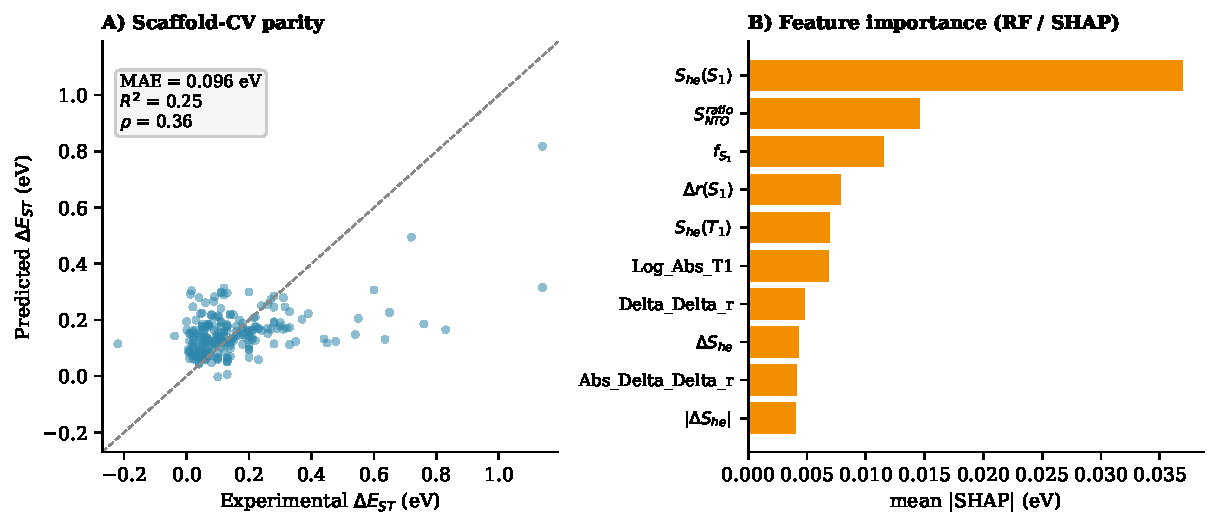
\includegraphics[width=0.95\textwidth]{figures/fig1_model_performance.pdf}
  \caption{Structure-based prediction of experimental $\Delta E_\text{ST}$.
    (A)~Scaffold cross-validated parity for the random forest on NTO
    spatial descriptors (\num{231} molecules, \num{212} Bemis--Murcko scaffolds):
    MAE = \qty{0.096}{\electronvolt}, $R^2 = 0.25$, Spearman $\rho = 0.36$. Models
    built from 2D structure alone (Morgan, RDKit) have similar errors
    (\cref{tab:feature_comparison}); formal equivalence was not established. The
    model regresses high-gap outliers toward the mean, the expected behaviour
    when the training distribution is dominated by low-gap emitters.
    (B)~SHAP importances: hole--electron overlap $S_\text{he}$, NTO overlap ratio,
    oscillator strength $f_{S_1}$ and charge-transfer distance $\Delta r$ dominate,
    consistent with exchange-integral physics.}
  \label{fig:model_performance}
\end{figure*}

We assembled \num{231} donor--acceptor molecules for which an experimental
$\Delta E_\text{ST}$ could be matched to a structure, and evaluated random-forest
regressors under Bemis--Murcko scaffold cross-validation (\num{212} distinct
scaffolds), so that no scaffold appears in both training and test.
Because \qty{92.9}{\percent} of scaffolds are singletons, scaffold and random splits
produce numerically similar folds (test--train nearest-neighbour Tanimoto differs by
only \num{0.022}). The scaffold split guarantees zero shared scaffolds per fold
(versus \numrange{3}{8} under a random split) but task difficulty barely changes;
the harder test of transfer is the source-paper split reported below.
That the model learns real signal rather than
scaffold-group structure is confirmed by a label-permutation test: the true
scaffold-CV MAE (\qty{0.096}{\electronvolt}) lies far below the null from
\num{1000} target shuffles (mean \qty{0.121}{\electronvolt}, $p = 0.001$;
Table~\ref{SI-tab:scaffold}).
The headline accuracy is also stable across validation schemes: replacing the singleton
scaffolds with genuine multi-molecule Butina clusters (down to \num{70} groups, largest
\num{38} molecules) leaves the MAE at \qtyrange{0.099}{0.104}{\electronvolt}, between
scaffold-CV (\qty{0.096}{\electronvolt}) and random-CV (\qty{0.106}{\electronvolt})
while preserving the rank correlation (Spearman $\rho$ spanning \numrange{0.31}{0.40} across cutoffs), showing that the ranking capability does not degrade under aggressive clustering
(Table~\ref{SI-tab:clustercv}).
The three feature sets perform within \qty{0.009}{\electronvolt} of one another
(\cref{tab:feature_comparison}); for the fingerprint and excited-state models, which we
compare head to head below, that closeness is backed by a paired bound of
\qty{0.017}{\electronvolt}. Two are computed from the 2D structure alone, with
no quantum chemistry: Morgan fingerprints (MAE = \qty{0.091}{\electronvolt}) and
RDKit physicochemical descriptors (\qty{0.100}{\electronvolt}). The third, NTO spatial
descriptors, is derived from a semi-empirical sTDA excited-state calculation but
excludes the $S_1$/$T_1$ energy scalars; it reaches MAE = \qty{0.096}{\electronvolt}
(\qty{95}{\percent} CI \numrange{0.082}{0.109}), $R^2 = 0.25$ (CI
\numrange{0.03}{0.45}), Spearman $\rho = 0.36$.
That the tested structure-only sets have similar errors to the NTO set is the
central comparison: the semi-empirical calculation has no measured error
advantage on these folds. Adding back the $S_1$/$T_1$ energies does not improve
the forest's MAE either (\cref{tab:feature_comparison}). The \emph{Energies~+~NTO}
set has MAE \qty{0.097}{\electronvolt} versus
\qty{0.096}{\electronvolt} for NTO alone. Similar predictive errors do not
establish that the feature sets encode identical physical information.
The natural comparator is the mean-value baseline (MAE = \qty{0.107}{\electronvolt}),
over which every model improves by only about \qty{10}{\percent}; the large apparent
gain over the raw sTDA gap (\qty{0.25}{\electronvolt}) reflects that the semi-empirical
gap is badly biased, not that the model is accurate.
The $R^2$ confidence intervals are wide and, for the structure-only sets, include
negative values (RDKit \numrange{-0.11}{0.51}; Morgan \numrange{-0.19}{0.53}): at
\qty{95}{\percent} confidence we cannot exclude that these models are no better than
predicting the mean. The signal is real but weak.

A higher level of theory does not change this picture. A range-separated TD-DFT
gap (wB97X-D4/def2-SVP, Tamm--Dancoff, \num{609} core-hours) overestimates the
measured gap by a systematic \qty{0.65}{\electronvolt} and, used directly, is the
least accurate predictor in \cref{tab:feature_comparison} (MAE
\qty{0.654}{\electronvolt}, $R^2 = -16.3$). Its correlation with experiment is
higher than the semi-empirical gap's (Pearson $r$ from \num{0.32} to \num{0.43}),
and an in-fold linear calibration that removes the offset brings it to MAE
\qty{0.099}{\electronvolt}---level with the mean-value baseline, still short of
the structure-only forest. Added as a single feature it lowers the Morgan model
from \num{0.091} to \qty{0.087}{\electronvolt} (paired \qty{95}{\percent} CI
\numrange{0.0004}{0.0071}, Wilcoxon $p = 0.016$): a small gain for
\num{609} core-hours (Table~\ref{SI-tab:tddft_headtohead}). This higher-level
TD-DFT descriptor is distinct from the semi-empirical NTO spatial set: the
latter does not lower the scaffold-CV error, whereas the former yields a
measurable but modest improvement.

Holding out whole source papers rather than scaffolds tests a different axis:
it removes entire publications and correlated chemical series. Because the corpus
records no measurement conditions per value, this is a proxy for shared practices,
not a laboratory- or protocol-controlled experiment. Under DOI-grouped five-fold
\texttt{GroupKFold} (\num{173} papers, \num{231} molecules) the Morgan model reaches
MAE \qty{0.102}{\electronvolt} ($R^2 = 0.18$; NTO $R^2 = 0.142$), and its paired advantage over the
mean-value baseline falls to \qty{0.005}{\electronvolt} with a \qty{95}{\percent}
CI that crosses zero. On accuracy, the model's advantage is not resolved under
this source-paper split.

Ranking behaves differently in these same folds: on this fixed fold assignment the NTO model has Spearman
$\rho = \num{0.35}$ while Morgan has \num{0.16} (MAE
\qty{0.099}{\electronvolt} against \qty{0.102}{\electronvolt}). Their paired
$\Delta\rho = \num{0.19}$ (the fixed-split value; the median over \num{50} random fold assignments is \num{0.16}, \cref{subsec:holdout_unit}) has a molecule-resampled \qty{95}{\percent} CI of
\numrange{0.04}{0.34}. Resampling the \num{173} primary source DOIs instead
gives \numrange{0.014}{0.366}; that paper-cluster interval barely excludes zero
and remains conditional on these fitted out-of-fold predictions. In \num{20}
additional paper-group partitions, retraining both models with \qty{20}{\percent}
of DOI groups held out each time, NTO has the higher test-set rank correlation
in \num{19} (median $\Delta\rho = \num{0.134}$; range
\numrange{-0.014}{0.404}). Those overlapping same-corpus partitions show
sensitivity to grouping rather than independent replication. Together these
tests identify a possible NTO ranking use case, not an advantage established
for selection in a new laboratory. One observation bounds the pessimistic reading, with a caveat that must travel with it:
\qty{58}{\percent} of repeatedly-measured molecules have zero inter-report spread, and
on the \num{102}-molecule multi-report subset the model reaches the study's lowest MAE,
\qty{0.080}{\electronvolt}. That subset is also an easier target: a mean-value predictor
restricted to it scores \qty{0.089}{\electronvolt}, so the model's advantage there is
\qty{0.009}{\electronvolt} with a \qty{95}{\percent} CI spanning zero. The low absolute
error reflects the narrower spread of those labels more than any gain in prediction.

\begin{table*}[t]
  \centering
  \caption{Prediction of experimental $\Delta E_\text{ST}$ under scaffold
    cross-validation (random forest, \num{231} molecules); $R^2$ with \qty{95}{\percent}
    bootstrap CI. The 2D-structure-only sets (no quantum chemistry) match the
    NTO set, which requires an sTDA excited-state run; none approaches the
    precision a quantitative photophysical method would require, and the
    structure-only $R^2$ intervals include zero. The range-separated TD-DFT
    reference gap (wB97X-D4/def2-SVP, Tamm--Dancoff; \num{609} core-hours) is
    listed raw, after an in-fold linear calibration, and as an added feature
    (Table~\ref{SI-tab:tddft_headtohead}).}
  \label{tab:feature_comparison}
  \begin{tabular}{lccc}
    \toprule
    Feature set & MAE (eV) & $R^2$ (\qty{95}{\percent} CI) & Spearman $\rho$ \\
    \midrule
    Morgan FP (2D structure only)   & 0.091 & 0.27 ($-0.19$, 0.53) & 0.31 \\
    RDKit desc.\ (2D structure only) & 0.100 & 0.31 ($-0.11$, 0.51) & 0.26 \\
    NTO spatial (needs sTDA)        & 0.096 & 0.25 (0.03, 0.45) & 0.36 \\
    Energies + NTO (reference)      & 0.097 & 0.24 & 0.34 \\
    \midrule
    Mean-value baseline             & 0.107 & 0.00 & --- \\
    Raw sTDA gap                    & 0.251 & $-2.22$ & 0.24 \\
    \midrule
    \multicolumn{4}{l}{\emph{Physics reference gaps (higher level of theory)}} \\
    Raw TD-DFT gap (wB97X-D4/def2-SVP) & 0.654 & $-16.3$ & 0.38 \\
    Calibrated TD-DFT gap (in-fold)    & 0.099 & 0.17 & 0.37 \\
    Morgan FP $+$ TD-DFT gap           & 0.087 & 0.31 & 0.37 \\
    \bottomrule
  \end{tabular}
\end{table*}

For the NTO variant, SHAP (SHapley Additive exPlanations) analysis
(\cref{fig:model_performance}B) identifies
hole--electron overlap $S_\text{he}$ (which governs the magnitude of the exchange interaction), the NTO overlap ratio (tracking transition purity), oscillator strength
$f_{S_1}$ (a proxy for transition dipole coupling), and the charge-transfer distance $\Delta r$ (which dictates spatial separation) as the dominant
predictors---physical quantities that jointly constrain the exchange integral governing
$\Delta E_\text{ST}$. This ranking is stable rather than an artefact of one fit:
across \num{200} bootstrap refits the leading descriptor $S_\text{he}(S_1)$ stays
in the top five \qty{99.5}{\percent} of the time, and on average \num{3.7} of the
five canonical descriptors recur (Table~\ref{SI-tab:shapboot}). Restricting the attribution to
the reliable-prediction subset---the \num{152} molecules whose out-of-fold residual is
below \qty{0.10}{\electronvolt}---leaves $S_\text{he}(S_1)$ ranked first in
\qty{99.5}{\percent} of refits, so the leading attribution does not rest on the
poorly-predicted tail. An independent, model-agnostic permutation-importance analysis ranks the same
descriptor, $S_\text{he}(S_1)$, first, so the leading attribution is corroborated by
two methods (the lower-ranked tail is not; SI section~S6.3). Given the model's modest
ranking power, we read only the dominant attribution as a mechanistic hypothesis for
experimental test rather than a validated causal claim; the structure-only
fingerprint and descriptor models reach the same accuracy without any excited-state
calculation.

\subsection{NTO and fingerprint models have similar error under scaffold holdout}\label{subsec:nto_null}

Do quantum-mechanical features beat pure structural descriptors when the target is an
experimental property? In scaffold cross-validation the tested NTO representation
does not reduce error. Paired on identical folds, the NTO model (MAE
$= \qty{0.096}{\electronvolt}$) and the Morgan model
($\qty{0.091}{\electronvolt}$) differ by
$\Delta\text{MAE} = \qty{-0.0043}{\electronvolt}$ for Morgan minus NTO
(\qty{95}{\percent} CI \numrange{-0.0171}{+0.0092}, Wilcoxon $p = 0.66$).
The lower confidence limit is close to the proposed
\qty{0.017}{\electronvolt} equivalence margin; we report the observed
similarity rather than claim a formal equivalence test. Both outperform the
mean-value baseline in paired comparisons, but neither predicts individual
gaps with the precision needed for emitter selection.

The accuracy comparison does not settle ranking on source-paper holdouts. In the
DOI-grouped folds (\cref{subsec:benchmark}), NTO retains Spearman
$\rho = 0.35$ while Morgan has $\rho = 0.16$; their paired difference on this fixed
fold assignment is $\Delta\rho = 0.19$ (paper-cluster \qty{95}{\percent} interval
\numrange{0.014}{0.366}), and the median over \num{50} fold assignments is
\num{0.16} (\cref{subsec:holdout_unit}). In a separate scaffold-CV triage analysis, at the
top \qty{20}{\percent} of the labelled benchmark NTO enrichment is
\num{1.6}-fold versus \num{1.4}-fold for Morgan.
The next subsection tests whether this ranking contrast comes from the evaluation
criterion or from the holdout unit. It does not establish that the contrast persists on
independent corpora or controlled protocols.
Recent theoretical work by Salvi et al.~\cite{Salvi2025} on electronic correlation
suggests a possible limitation of semi-empirical descriptors; the present
comparison alone cannot identify its cause.
The two representations differ in what they can be read for, though not in a way the
attribution totals establish on their own. The ten highest-attribution NTO descriptors
carry \qty{79}{\percent} of that model's SHAP weight against \qty{30}{\percent} for the
ten highest-attribution Morgan bits (Figure~\ref{SI-fig:shapcompare}); those totals are not
comparable, because ten descriptors are \qty{29}{\percent} of the \num{35}-dimensional
NTO set and ten bits are \qty{0.5}{\percent} of a \num{2048}-bit fingerprint, so the
concentration follows from dimensionality. What does not follow from dimensionality is
that the NTO features are \emph{named} donor--acceptor overlap and charge-transfer
quantities, whereas Morgan bits are anonymous hashed substructures. The case for the
physics-informed representation is interpretability of the variables themselves, not a
larger share of attribution.

\subsection{Fingerprint ranking depends on same-publication molecules}\label{subsec:holdout_unit}

The holdout unit, not the error-versus-ranking criterion, sets the size of the NTO--Morgan rank
contrast. We repeated the comparison with \num{50} random assignments of groups to five folds for
each of three units (\cref{tab:holdout_unit}). Under source-paper holdout the median
$\Delta\rho$ (NTO minus Morgan) is \num{0.160} and is positive in \num{50} of \num{50} assignments;
under scaffold holdout it is \num{0.073} (\num{49}/\num{50} positive) and under random
molecule holdout \num{0.055} (\num{45}/\num{50} positive). The \num{0.191} of the fixed
split lies in the upper part of the paper-holdout distribution, so the fold-assignment-robust
value is $\approx\num{0.16}$ (\num{50}-assignment range \numrange{0.07}{0.25}); the ranges
describe fold-assignment variability, not confidence intervals. The error comparison does not move
with the unit: Morgan minus NTO MAE is \qty{-0.0004}{\electronvolt} under paper holdout and
\qty{-0.0045}{\electronvolt} under scaffold holdout, with ranges that span zero, and
\qty{-0.0081}{\electronvolt} under random holdout, where Morgan is slightly better
(range \numrange{-0.0157}{-0.0002}). NTO is higher in \num{19} of \num{20} repeated
paper-group partitions, against \num{11} of \num{20} for scaffold and \num{13} of \num{20}
for molecule partitions, so the earlier \num{19}/\num{20} count is specific to the paper unit.

\begin{table}[htbp]
  \centering
  \caption{Rank correlation of random-forest models by holdout unit (same \num{231}
    molecules; \num{50} random group-to-fold assignments, medians). $\Delta\rho$ is NTO minus Morgan;
    the range is the 2.5th to 97.5th percentile over assignments, a measure of
    fold-assignment variability, not a confidence interval. The last column counts
    \num{20} repeated holdout partitions in which NTO has the higher test-set $\rho$.
    RDKit 2D descriptors were run under molecule and paper holdout only (n.t., not tested);
    their multi-paper $\rho$ falls from \num{0.518} to \num{0.350} and single-paper $\rho$ under
    paper holdout is \num{0.102}.}
  \label{tab:holdout_unit}
  \footnotesize\setlength{\tabcolsep}{1.5pt}
  \begin{tabular}{lcccccc}
    \toprule
    & & & \multicolumn{3}{c}{median $\rho$} & NTO \\
    \cmidrule(lr){4-6}
    Unit (groups) & $\Delta\rho$ & Range & Morgan & RDKit & NTO & higher \\
    \midrule
    Paper (\num{173})    & 0.160 & 0.073--0.246 & 0.172 & 0.209 & 0.337 & 19/20 \\
    Scaffold (\num{212}) & 0.073 & 0.007--0.144 & 0.269 & n.t. & 0.351 & 11/20 \\
    Molecule (\num{231}) & 0.055 & $-0.033$--0.126 & 0.305 & 0.303 & 0.352 & 13/20 \\
    \bottomrule
  \end{tabular}
\end{table}

The contrast comes from the fingerprint side. NTO rank correlation is nearly invariant to the unit
(median $\rho$ \numrange{0.337}{0.352}), whereas Morgan $\rho$ falls from \num{0.305} (random) to
\num{0.269} (scaffold) to \num{0.172} (source paper) (\cref{fig:holdout_unit}a). Splitting the
molecules by paper multiplicity locates the drop (\cref{fig:holdout_unit}b). For the \num{103}
molecules whose paper contributes at least one other molecule, Morgan $\rho$ is \num{0.54} when
siblings are in training and \num{0.26} when the whole paper is held out, while NTO moves from
\num{0.48} to \num{0.45}. For the \num{128} molecules from single-molecule papers, Morgan $\rho$ is
\num{0.10} under either holdout against \num{0.24} for NTO; with predictions averaged over the
\num{50} paper-holdout assignments the two are \num{0.11} and \num{0.27}, a difference of
\num{0.16} whose paired bootstrap \qty{95}{\percent} CI (\numrange{-0.05}{0.37}) includes zero,
so this subset contrast is not resolved. The sibling-pull statistic, the Spearman
correlation between a molecule's prediction and the mean label of its same-paper siblings, is
\num{0.68} for Morgan under random holdout and \num{0.26} under paper holdout, against \num{0.47} and
\num{0.42} for NTO. Morgan's MAE on multi-paper molecules is \qty{0.025}{\electronvolt} lower under random
than under paper holdout (range \numrange{0.014}{0.034}); NTO's difference is
\qty{0.007}{\electronvolt}, with a range that includes zero.

A dense descriptor set without quantum chemistry behaves like the fingerprint. The \num{217}
RDKit 2D descriptors, run through the same \num{50} assignments, reach median $\rho$ \num{0.303}
under random and \num{0.209} under paper holdout; on multi-paper molecules $\rho$ falls from
\num{0.518} to \num{0.350}, and on single-paper molecules it is \num{0.102}
(\cref{tab:holdout_unit}). Among the three sets tested, holdout-unit invariance is specific to
the NTO descriptors, and dimensionality alone does not explain it. None of the three orders
molecules \emph{within} a held-out paper: the Spearman correlation between paper-centred labels and
paper-centred predictions on the \num{103} multi-paper molecules is \num{-0.06} to \num{0.03}
under paper holdout. The NTO advantage is in ordering emitters across publications absent from
training. Under random holdout Morgan's within-paper $\rho$ is \num{-0.35}: its predictions are
pulled towards the sibling mean, which inverts the order inside a paper.

\begin{figure}[t]
  \centering
  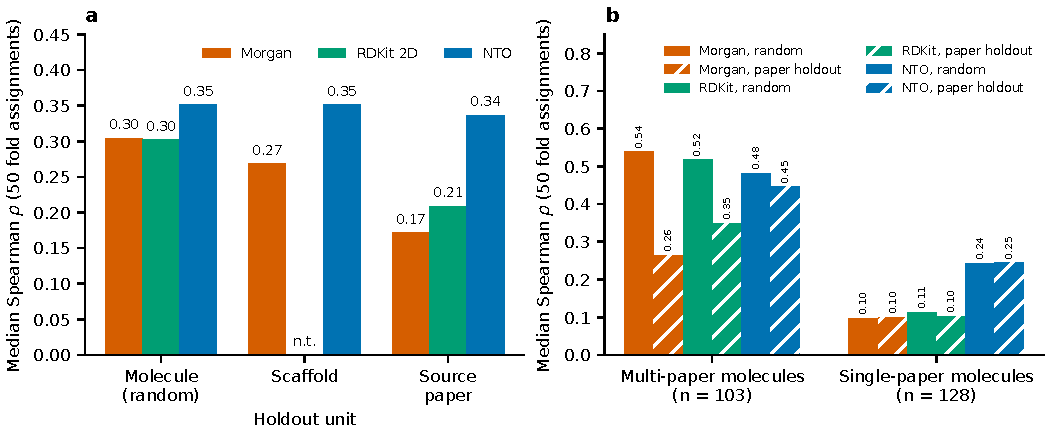
\includegraphics[width=\columnwidth]{figures/holdout_unit_ranking.pdf}
  \caption{Rank correlation by holdout unit and by paper multiplicity (medians over \num{50} random
    fold assignments; random-forest models on the same \num{231} molecules). (a)~Spearman $\rho$ for
    Morgan, RDKit 2D and NTO features under molecule, scaffold and source-paper holdout (RDKit was
    not run under scaffold holdout; n.t.). (b)~$\rho$ for the \num{103} molecules from
    multi-molecule papers and the \num{128} from single-molecule papers, under random and paper
    holdout. The full seed-range tables are in the SI.}
  \label{fig:holdout_unit}
\end{figure}

This is an association. Molecules from one paper share close structure and measurement protocol,
and these tests cannot separate structural near-duplication from laboratory or protocol effects. The
paper-multiplicity test compared random with source-paper holdout only (scaffold holdout was not
part of it): the fingerprint model's ranking skill under random holdout sits mostly on molecules whose
same-paper siblings are in training, and the NTO descriptors keep their rank information when
the siblings are absent. All units use one corpus and \num{128} of the \num{173} papers contribute a
single molecule, so paper holdout differs from random holdout through the \num{45} multi-molecule papers
only; no test here crosses laboratories.

\subsection{Label scatter leaves the ceiling at $R^2_\text{max} \approx 0.8$, well above the observed $R^2$}\label{subsec:ceilings}

The observed MAE is near \qty{0.1}{\electronvolt}, but label variability does
not by itself account for the model's error.
Independent experimental reports for the same compound disagree
substantially: a single randomly chosen report sits \qty{0.072}{\electronvolt} from its
molecule's median (RMS with each molecule weighted equally), the disagreement exceeds the
model MAE for \qty{19.6}{\percent} of molecules, and the worst molecule reaches a standard
deviation of \qty{0.56}{\electronvolt}; the eight independent values for 4CzIPN alone span
\qtyrange{0.01}{0.48}{\electronvolt} (Table~\ref{SI-tab:solvent}). This scatter is consistent with uncontrolled measurement conditions (solvent polarity, concentration, host matrix), which influence photophysical measurements~\cite{Dang2025}; the corpus cannot separate conditions, protocol and transcription error. That $\Delta E_\text{ST}$
is reported inconsistently has been shown for individual emitters~\cite{Shuaib2026};
quantified across \num{231} molecules and \num{173} source papers it provides
an inter-report variability estimate for this TADF corpus. This variability
constrains any predictor fitted to the measured labels.
The quantity the model is regressed on, however, is the per-molecule \emph{median}.
For the \num{102} molecules with several reports, the RMS standard error of that median
is \qty{0.049}{\electronvolt}; the other \num{129} labels rest on one report each, and
counting them at single-report scatter gives an RMS label noise of about
\qty{0.072}{\electronvolt} over all \num{231} molecules. Label imprecision is therefore
a real term in the error budget but does not by itself account for it, and we do not
claim the forest sits at a noise floor.
Applying the noise-ceiling framework of Crusius et al.~\cite{Crusius2025}
($R^2_\text{max} = 1 - \sigma^2_\text{noise}/\sigma^2_y$) with per-molecule noise
(the standard error of the mean for the \num{102} multi-report molecules, and the
single-report scatter for the \num{129} single-report molecules) gives
$R^2_\text{max} \approx 0.81$ (\qty{95}{\percent} CI \numrange{0.68}{0.88}) for the
pooled within-molecule SD of \qty{0.0856}{\electronvolt}; the alternative single-report
estimates give \num{0.80} and \num{0.86}. All lie well above the observed $R^2 \approx 0.26$.
The model captures about \qtyrange{30}{32}{\percent} of that ceiling, so label noise alone is not the dominant
constraint. The assumptions behind the ceiling are listed in SI section~S3.3b.
Progress requires both a better dataset \emph{and} improvements in features or
corpus scale; label noise (about \qty{0.072}{\electronvolt} RMS over the \num{231}
molecules) is the term a curated benchmark would directly attack.
A second, separate dispersion applies to computed references rather than to this
regression: the computed gap is functional-dependent. Across the
\num{7} molecules (gas and toluene) for which we ran both B3LYP/6-31G(d) and CAM-B3LYP/def2-TZVP,
$\Delta E_\text{ST}$ differs by a mean \qty{0.30}{\electronvolt} (up to
\qty{0.58}{\electronvolt}) and changes
relative magnitude (Table~\ref{SI-tab:dft_benchmark}); a higher-tier benchmark across
six range-separated functionals on \num{27} emitters~\cite{Froitzheim2024} shows the same
effect at finer resolution: a median inter-functional spread of \qty{0.05}{\electronvolt}
on a quantity that approximates \emph{half} the gap, hence roughly
\qty{0.1}{\electronvolt} on \deltaest\ itself. Any claim of sub-\qty{0.1}{\electronvolt}
accuracy against such a reference is not physically meaningful. This second effect bounds
what a \emph{computed} gap can mean; it does not bound a model regressed on measured
labels, and we do not add the two into a single floor. Only the label term applies
directly to the present task. Among the representations tested here, larger
learner capacity does not close the gap. Histogram gradient boosting reaches
\qty{0.105}{\electronvolt}, an MLP \qty{0.169}{\electronvolt} and an RBF SVR
\qty{0.120}{\electronvolt} (Table~\ref{SI-tab:capacity}); a second comparison over a
differently configured set of learners places plain gradient boosting at
\qty{0.098}{\electronvolt}, within \qty{0.002}{\electronvolt} of the forest and well below the proposed
\qty{0.017}{\electronvolt} comparison margin
(Table~\ref{SI-tab:capacity} lists the
histogram-boosting configuration). A frozen pretrained SMILES transformer (ChemBERTa,
\num{77}M parameters), the representation a current screening pipeline would reach for
first, is no exception: its mean-pooled embeddings feed a random-forest or ridge head
to MAE \qtyrange{0.109}{0.113}{\electronvolt} on the same scaffold folds---it does not
beat the \qty{0.107}{\electronvolt} mean-value baseline, and is worse than Morgan by a
paired \qty{0.022}{\electronvolt} (\qty{95}{\percent} CI \numrange{0.008}{0.034},
excluding zero; \texttt{code/a013\_pretrained\_encoder\_baseline.py}). Fine-tuning this encoder on only \num{231} labels was not tested here.
Among the representations evaluated, added capacity did not improve the
measured-gap error; this does not exclude other architectures or training sets.
The negative lower $R^2$ bound is not a
fingerprint-width artefact, since \num{512}-, \num{1024}- and \num{2048}-bit Morgan models
share it (Table~\ref{SI-tab:capacity}).

Stratifying by label quality does not isolate a label effect. Restricting to molecules that carry replicates, the model reaches MAE
\qty{0.074}{\electronvolt} on the \num{79} whose reports agree to
$\le\qty{0.05}{\electronvolt}$, \qty{0.106}{\electronvolt} on the \num{23} whose
reports do not, and \qty{0.107}{\electronvolt} on the \num{129} for which label
precision cannot be measured. That ordering is not evidence about labels: a constant
predictor fitted within each stratum reproduces it almost exactly
(\qty{0.074}{}, \qty{0.107}{} and \qty{0.110}{\electronvolt}), because the strata
differ in the dispersion of the target itself (standard deviation \qty{0.10}{},
\qty{0.15}{} and \qty{0.20}{\electronvolt}). Within any one stratum the model carries
no advantage over a constant. We therefore report no stratified evidence for a label
ceiling; the quantitative statement that survives is the label-noise estimate above.

A related question is whether \emph{uncontrolled measurement conditions}, rather than
label imprecision as such, set the limit. The corpus records no solvent, host or
temperature for individual values, so a strictly condition-controlled subset cannot be
built; the closest available grouping is by source paper, without a guarantee that
measurements in one publication share a laboratory or solvent. Splitting the benchmark on that
(\num{218} single-source against \num{13} multi-source molecules) and scoring the random
forest on scaffold cross-validation folds, the model's descriptive advantage
over a constant fitted within each full group is \qty{0.0071}{} and
\qty{0.0024}{\electronvolt}, respectively. The latter comparator is not held out:
a separate out-of-fold recalculation gives \qty{0.1006}{\electronvolt} and
\qty{0.0693}{\electronvolt} for the single- and multi-source groups. The old
group-difference interval (\numrange{-0.014}{0.035}) used the in-sample constants
and must not be interpreted as a matched predictive comparison. The raw
errors run the other way (\qty{0.058}{} against \qty{0.093}{\electronvolt}) but the
multi-source group's target dispersion is half as large and its in-sample constant
scores \qty{0.061}{\electronvolt}; the held-out constant scores
\qty{0.069}{\electronvolt} instead. With only \num{13} molecules drawing on
more than one source paper, neither a benefit nor a penalty of mixed source
membership is resolved by these comparisons. The corpus does not permit a
controlled test of solvent or measurement protocol.

A larger but differently processed corpus gives a stress test, not an isolated
sample-size experiment. Featurising \num{497} additional
experimental emitters through the same pipeline (a \num{728}-molecule set) raises
the MAE from \qty{0.098}{} to \qty{0.124}{\electronvolt}, drives $R^2$ from
\num{0.18} to $-0.01$, and roughly halves the rank correlation (Spearman $\rho$
from \num{0.34} to \num{0.16}); the replicate-measured subset
($n = \num{465}$) recovers only about half of the loss (Table~\ref{SI-tab:expansion}).
In this expanded, differently processed set, prediction worsens rather than
improves. The added molecules were resolved through a different structure
pipeline, so broader chemistry, target quality, and preprocessing are confounded;
the comparison cannot determine whether corpus size alone helps or hurts.

A separate concern is the descriptor side: the NTO features are computed at the
\emph{vertical} (ground-state) geometry, whereas the measured gap reflects relaxed
excited states. We bounded this approximation by recomputing \deltaest\ adiabatically
for \num{14} representative emitters in gas and toluene at CAM-B3LYP/def2-TZVP with
excited-state optimisation (Table~\ref{SI-tab:adiabatic}). Relative to these adiabatic
references the vertical gap carries a mean absolute deviation of
\qty{0.195}{\electronvolt}, which exceeds the model's own error. The deviation is
dominated by an additive offset rather than by reordering---a linear fit gives slope
\num{1.00} and intercept \qty{0.07}{\electronvolt} ($R^2 = 0.70$, Spearman
$\rho = 0.71$)---so relaxation shifts the scale more than it scrambles the ranking the
triage relies on. The residual is not negligible, however: the RMS deviation is
\qty{0.245}{\electronvolt} and the worst molecule departs by \qty{0.548}{\electronvolt},
with sign changes between compounds, and \num{14} molecules cannot settle how much of
that is systematic. We take the vertical descriptors as an acceptable ranking input on
this evidence, not as a validated approximation to the adiabatic gap.

Candidate triage (enrichment \num{1.2}--\num{1.4}$\times$ over random for low-gap emitters,
established only at cutoffs of about \num{50} molecules or a fifth of the benchmark) and the
\num{22194}-structure substructure-filtered library, where split-conformal intervals rule out
single-molecule selection, are reported in SI section~S6.7.

\subsection{The cited TADF-gap models report error on computed gaps, not ranking across held-out publications}\label{subsec:comparison}

The low errors reported for TADF-gap models are obtained against computed targets:
a TD-DFT gap inside a $>$\num{1000000}-molecule screen~\cite{Gomez-Bombarelli2016},
semi-empirical gaps over a virtual library~\cite{Thapa2025}, ADC(2) gaps of
inverted-gap molecules reproduced to \qty{0.02}{\electronvolt}~\cite{Barneschi2024},
quasiparticle-corrected Kohn--Sham gaps for \num{233} INVEST and TADF molecules at
\qty{0.06}{\electronvolt}~\cite{Li2026}, and $\omega$B2PLYP$'$ gaps that Nigam
et al.\ moved from regression to a good/bad classifier~\cite{Nigam2024}
(Table~\ref{SI-tab:prior_ml}). He et al.~\cite{He2026} trained on \num{1321}
measured gap records with measurement-condition features but did not compare
fingerprint and semi-empirical NTO representations under molecule, scaffold and
source-publication holdout.
Against measured gaps, whose labels carry about \qty{0.072}{\electronvolt} RMS of
inter-report noise, the Morgan and NTO models reach \qtyrange{0.091}{0.096}{\electronvolt},
\qtyrange{10}{15}{\percent} below the mean-value predictor (naive baselines in
Table~\ref{SI-tab:baselines}). Whether the computed-gap estimators keep their
accuracy against measured gaps has not been tested, and none of these studies reports how ranking holds when whole publications are held out, the test made in \cref{subsec:holdout_unit}.

\subsection{Limitations}\label{subsec:limitations}

All results come from one corpus of \num{231} molecules, so the holdout-unit comparison does not
test transfer to a new laboratory or a controlled protocol. The target is a consensus
literature value (inter-report RMS scatter \qty{0.072}{\electronvolt}) of a single scalar,
$\Delta E_\text{ST}$; solvatochromic, conformer-dependent and device-level quantities are not
predicted. The NTO descriptors use ground-state vertical geometries (mean absolute deviation
\qty{0.195}{\electronvolt} from adiabatic references for \num{14} emitters), inverted-gap
emitters are out of scope (both negative labels receive positive predictions), and only
tabular learners and one frozen pretrained encoder were tested. Ranking is moderate
($\rho \approx 0.34$ to $0.36$), so the models support triage, not selection. The full list is in
SI section~S6.8.
